\chapter{发 绀}

发绀以往称为紫绀,是指血中含有过量的脱氧血红蛋白,致皮肤和黏膜出现广泛的青紫颜色。全身皮肤与黏膜均可出现发绀,但以口唇、舌、口腔黏膜、鼻尖、颊部、耳垂与指(趾)末端等皮肤薄、色素少和毛细血管网较丰富的部位最为明显。血中含有异常的血红蛋白衍化物(高铁血红蛋白、硫化血红蛋白),以及皮肤的异常色素或异物沉着(银质沉着症、金质沉着症等),也可出现皮肤青紫,但不应与真性发绀相混淆。此外,寒冷时小动脉的强烈收缩,也可引起局部发绀。

国外文献曾有报告儿童病例由于长期应用银剂滴鼻引起皮肤类似发绀色,被误诊为先天性心脏病。

发绀疾病的临床分类见表\ref{tab14-1}。\footnote{*正常每100ml血液中含血红蛋白约15g,能携带20容积\%的氧,在此情况下称为100\%氧饱和度。正常从肺毛细血管流经左心至体动脉的血液,其氧饱度约为96\%(相当于19容积\%),而静脉血液的氧饱和度为72\%~75\%(相当于14~15容积\%,即氧未饱和度为6~5容积\%);在周围循环的毛细血管血液中,氧的未饱和度平均约为3.5容积\%。当周围循环毛细血管血液中还原血红蛋白超过5g/100ml,即血氧未饱和度达到6.5容积\%或以上时,则出现发绀。但在重症贫血病人,如每100ml血液中血红蛋白量低于5g时,即使全部变为还原血红蛋白,也不至引起发绀}

\begin{longtable}{c}
 \caption{发绀疾病的临床分类}
 \label{tab14-1}
 \endfirsthead
 \caption[]{发绀疾病的临床分类}
 \endhead
 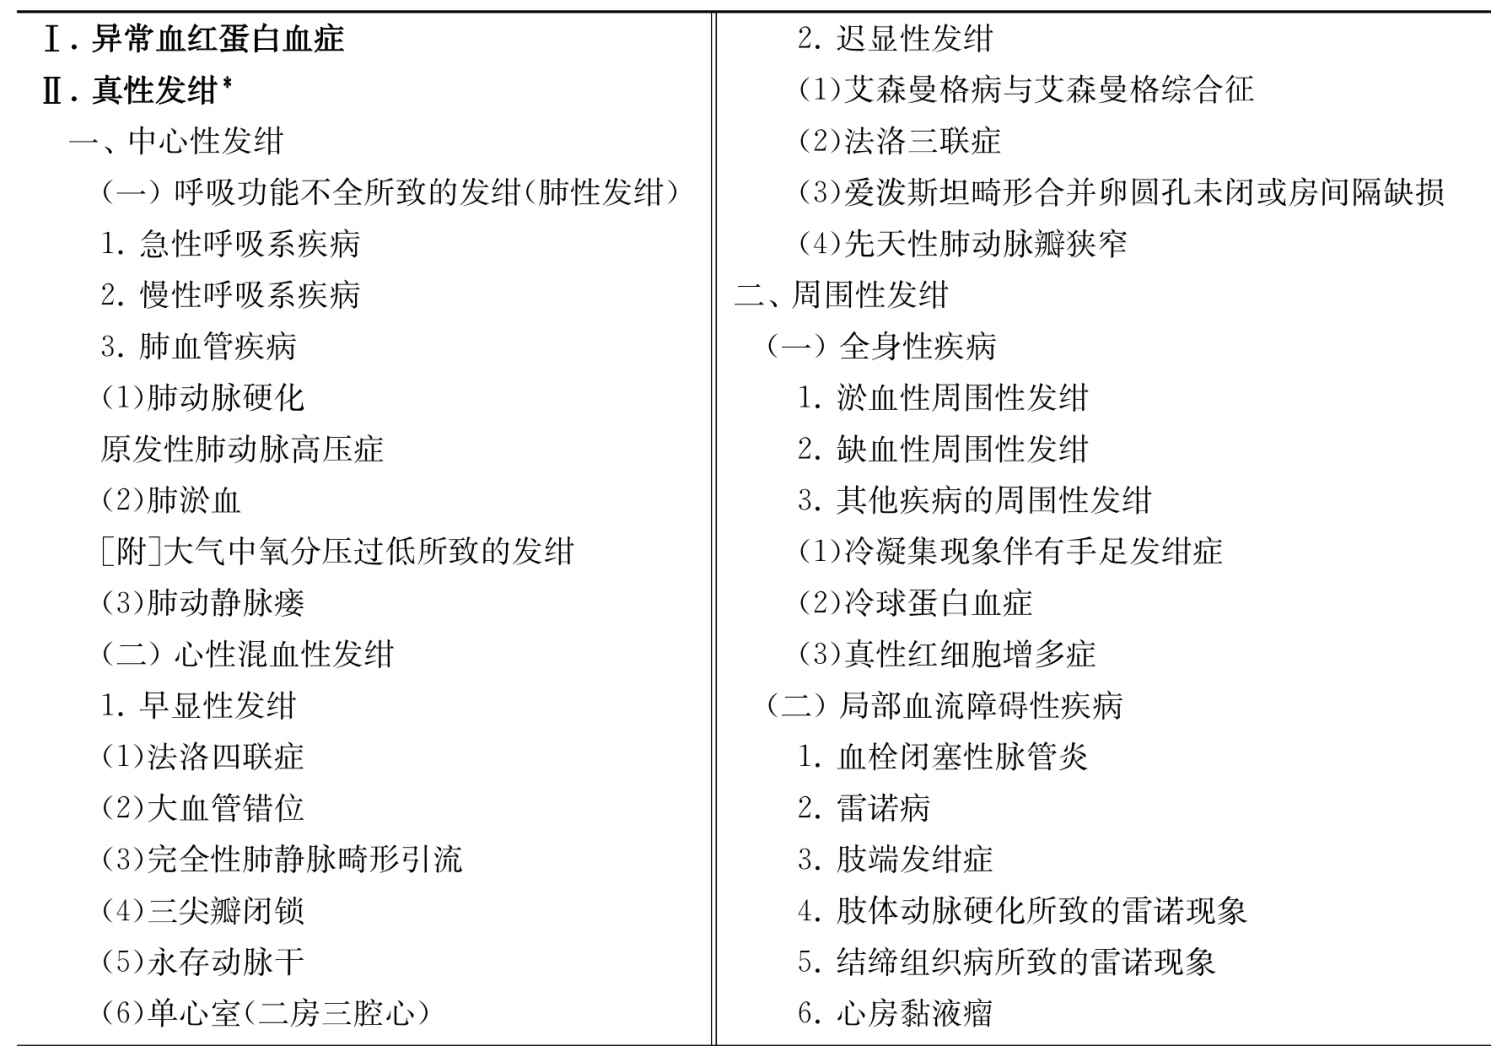
\includegraphics[width=\textwidth,height=\textheight,keepaspectratio]{./images/Image00091.jpg}\\
 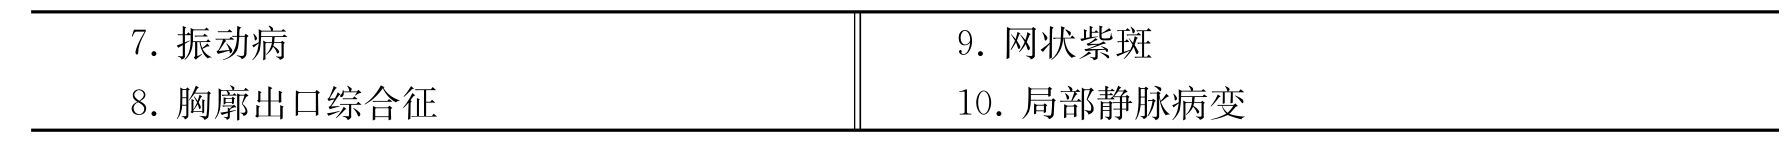
\includegraphics[width=\textwidth,height=\textheight,keepaspectratio]{./images/Image00092.jpg}
 \end{longtable}
 
血中还原血红蛋白增多可由于:①心、肺疾病所致的动脉血氧饱和度不足(中心性发绀);②周围循环血流障碍(周围性发绀)。如两者并存,则称为混合性发绀。

异常血红蛋白血症与真性发绀鉴别要点:

\section{(一)病史}

自出生时或幼年即出现发绀者,常为发绀类先天性心血管病,或先天性高铁血红蛋白血症。药物或化学物品中毒所致的高铁血红蛋白血症,常有明确的接触史。

\section{(二)体征}

重度的发绀,主要见于发绀类先天性心血管病、高铁血红蛋白血症、硫化血红蛋白血症、原发性肺动脉高压症与肺动静脉瘘。反复发作的肢端发绀,常由于局部循环障碍所致。急性发绀伴有衰竭状态或意识障碍。常见于某些药物或化学物品急性中毒、休克、急性肺部感染或急性充血性心力衰竭。发绀伴杵状指(趾),主要见于发绀类先天性心血管病(尤以法洛四联症)、原发性肺动脉高压症、肺动静脉瘘,也可见于某些慢性肺部疾病。一般后天性心脏病、急性呼吸道疾病、高铁血红蛋白血症与硫化血红蛋白血症,均无杵状指。心肺疾病的发绀常伴有高度的呼吸困难。高铁血红蛋白血症与硫化血红蛋白血症,发绀虽明显而一般并无呼吸困难。

\section{(三)器械与实验室检查}

高铁血红蛋白、硫化血红蛋白的检查,须依靠有关的实验室检查方法。发绀类先天性心血管病常须依靠心脏超声、心导管检查及(或)选择性心血管造影等方能确定诊断。

\protect\hypertarget{text00119.html}{}{}

\section{43 异常血红蛋白血症}

\subsection{一、药物或化学物品中毒所致的高铁血红蛋白血症}

在高铁血红蛋白血症时,血红蛋白分子的二价铁被三价铁所代替,致失去与氧结合的能力。血中高铁血红蛋白达1.5g/100ml时即引起发绀。

此型高铁血红蛋白血症并非太少见,严重者危及生命,通常由于服用伯氨喹、亚硝酸盐、氯酸钾、碱式硝酸铋、磺胺类、非那西丁、苯丙砜、多黏菌素B等引起,亦有报道利福平可导致发绀发生。非那西丁所致发绀多见于婴儿。在化学工业生产过程中不慎吸入或接触苯胺衍化物引起发绀者也有报告。也有报告见于烧伤患者。

此型高铁血红蛋白血症的特征性表现是:

1.发绀为暂时性。

2.发绀由于上述药物或化学物品所引起。

3.静脉血呈深棕色,暴露于空气中也不转变为鲜红色。加入硫代硫酸钠或维生素C后,可使高铁血红蛋白变为鲜红色的氧合血红蛋白。

4.静脉注射大量维生素C可使发绀显著减轻,而静脉注射亚甲蓝溶液(每公斤体重2mg)的效果尤为迅速,且为不可缺少的急救措施。

5.在红细胞内出现海涅茨(Heinz)小体。长期持续的高铁血红蛋白血症可引起溶血性贫血。

6.分光镜检查证明血内高铁血红蛋白的存在。

\subsection{二、肠源性发绀}

肠源性发绀是中毒性高铁血红蛋白血症的一种类型。国内报告的肠源性发绀大都由于进食过量含有亚硝酸盐的蔬菜所引起。患者多为2~10岁的儿童。亚硝酸盐在隔夜的煮熟青菜或盐腌不久的咸菜中含量尤多,体弱的人过多食用时则可致病,俗称为“菜紫乌”病。此病发病急骤,患者自觉头晕、倦怠、乏力、表情淡漠,继而口唇与肢端发绀,少数有呕吐、腹痛、腹泻等症状。严重者可因昏迷、休克而死亡。

误将亚硝酸钠作为食盐,用于烹调而致集体中毒者也时有报告。

\subsection{三、遗传性高铁血红蛋白血症}

此类疾病少见,血红素中的高铁不能还原成低铁,阻止了血红蛋白与氧结合,因而产生高铁血红蛋白致发绀,主要可分为二型:

\subsubsection{(一)NADH高铁血红蛋白还原酶(黄递酶)缺乏症}

本病属隐性遗传,发绀常于出生时即出现。患者虽有明显的发绀,而全身症状轻微,也无明显心肺疾病与杵状指。NADH黄递酶缺乏可经实验室检查而确定之。高铁血红蛋白的分光镜检查特点是在波长618~630nm外有一黑色吸收光带。亚甲蓝与维生素C治疗能使发绀缓解。

\subsubsection{(二)血红蛋白M病}

本病属显性遗传。据国内一组四个家系52个成员中,出生时即有发绀。本病时,发绀是唯一的明显临床表现,且自幼即出现。血红蛋白M的酸性高铁血红蛋白溶血产物,在分光镜下呈现特别的吸收光带,据此可与其他原因的高铁血红蛋白血症相区别。血红蛋白电泳也有诊断价值。亚甲蓝与维生素C治疗对血红蛋白M病的发绀均无疗效。

\subsection{四、特发性阵发性高铁血红蛋白血症}

此病并非家族性,可见于妇女,发绀出现与月经周期有关。此病国内尚无报告。

\subsection{五、硫化血红蛋白血症}

正常人血红蛋白中可有2\%硫化血红蛋白。能产生高铁血红蛋白的药物或化学物品,也能产生硫化血红蛋白,这些药物或化学物品主要是:①含氮化合物,如硝酸钾、亚硝酸钠等;②芳香族氨基化合物,如磺胺、苯胺衍生物、非那西丁等。生成硫化血红蛋白还需患者同时有便秘或服用硫化物(主要为含硫的氨基酸),在肠内形成大量硫化氢为先决条件;所服用的含氮化合物或芳香族氨基化合物则起触酶的作用,使硫化氢作用于血红蛋白,而生成硫化血红蛋白。血中硫化血红蛋白达0.5g/100ml时则引起发绀。

硫化血红蛋白呈蓝褐色,故患者的主要症状是发绀。硫化血红蛋白一经合成,不论在体内或体外都不能恢复为血红蛋白。含硫化血红蛋白的红细胞寿命仍属正常,如一旦发生发绀,发绀持续时间很长。

欲证明高铁血红蛋白与硫化血红蛋白,可于被检者全血中加入适量蒸馏水使成1∶10~100的稀释液,取此溶血稀释液各数毫升分置于两个试管中,第一管在分光镜下检查,如为高铁血红蛋白,于光谱红色区域的630nm处出现吸收光带;第二管加入5\%氰化钾溶液数滴,如为高铁血红蛋白则吸收光带消失。硫化血红蛋白于620nm处出现一吸收光带,在分光镜下难与高铁血红蛋白区别,但加入氰化钾后此吸收光带不消失。如加入3\%H\textsubscript{2}
O\textsubscript{2}
,则使高铁血红蛋白与硫化血红蛋白二者的吸收光带均消失。

硫化血红蛋白血症国内曾有一例报告,此例发绀持续多年。

\protect\hypertarget{text00120.html}{}{}

\section{44 真性发绀}

还原血红蛋白增多所致的发绀(真性发绀),根据其病因可分为中心性和周围性两大类,分述于下:

\subsection{44.1 中心性发绀}

中心性发绀的发病机制主要有两方面:

1.肺通气或换气功能的障碍,由于:①呼吸道梗阻;②肺小动脉硬化;③广泛性呼吸面积减少所致的呼吸功能不全,如肺不张、重症肺结核、肺炎、肺淤血、硅沉着症等。

2.血液在肺内达到正常的氧饱和度,但在流入左心后混有大量静脉血,如房间隔缺损、室间隔缺损、Lutembacher综合征等有相反方向的分流时。

根据临床特点,中心性发绀又可区分为肺性与心性混血性发绀两类。二者的主要鉴别根据是:

\subsubsection{1.病史、体征}

前者有肺病病史及体征;后者有心脏病史及体征。

\subsubsection{2.肺性发绀}

有呼吸功能不全的存在通常依靠简单的吸氧试验即能得出重要的鉴别根据。在呼吸功能不全时,患者吸入纯氧5~10分钟后,可使发绀明显减轻或甚至消失,如在吸氧前后作血氧含量测定,则能获得更明确的指标。

\subsubsection{3.心性混血性发绀}

常有心内分流的存在,彩色多普勒超声是最有价值的无创诊断方法,一般可明确诊断,必要时可行心导管检查术。

\subsubsection{44.1.1 呼吸功能不全所致的发绀(肺性发绀)}

此类疾病包括急性或慢性呼吸系疾病、肺血管疾病(如肺动脉硬化、原发性肺动脉高压症)及肺淤血等,分述于下:

\paragraph{一、急性呼吸系统疾病}

在喉头或气管梗阻、支气管哮喘发作等情况时,进入肺泡的空气减少,肺泡内氧分压降低,肺毛细血管血氧饱和度不足,可引起发绀。大叶性肺炎、弥散性或大面积肺梗塞时,由于肺呼吸面积减少,致动脉血氧饱和不足,也可引起发绀。

\paragraph{二、慢性呼吸系统疾病}

累及胸膜、肺或支气管的重症慢性疾病(肺结核病、矽肺、支气管扩张、慢性支气管炎等),由此引起的慢性梗阻性肺气肿,以及由于脊柱后侧凸所致的胸廓畸形等,均常引起轻度发绀,但其严重程度远不及原发性肺动脉高压症。患者的呼吸困难大多明显。根据慢性肺部疾病的存在,诊断常无困难。

\paragraph{三、肺血管疾病}

\subparagraph{(一)肺动脉硬化}

重症肺动脉硬化时,病变累及较大和细小的肺动脉,严重的管腔狭窄妨碍血流的通过。由于肺动脉血压显著升高,长期加重右心的负担,引起右心室扩张与肥厚。当右心室衰竭出现时,发绀可因此而加重。

心脏呈肺源性心脏病的改变,肺动脉瓣第二音高度增强,右心室扩大与肥厚,心电图显示右心室肥厚、电轴右偏。X线检查肺野清晰,与浓厚的肺门阴影呈明显的对比。

原发性肺动脉高压症(Ayerza病):此病是一种肺小动脉的进行性狭窄性与阻塞性变,病因常为先天性异常。此病少见,临床诊断相对困难。自心血管造影术检查和超声心动图开展以来,临床确诊病例渐多报告。此病的四大特点是:慢性发绀、呼吸困难、红细胞增多与右心衰竭;咯血与晕厥也常见。

原发性肺动脉高压症与慢性肺部疾病(肺气肿、结核病、支气管扩张)所致的继发性肺动脉高压症鉴别有困难,因二者的临床表现相似,病史有重要参考价值。

体格检查在胸骨左缘第2~4肋间有时可听到较粗糙的收缩期杂音,X线检查右心室增大与肺动脉扩张,心电图显示右心室肥厚,在此情况下与伴有肺动脉高压的先天性心脏病从临床症状鉴别确有困难,但原发性肺动脉高压症一般具有重度发绀而呼吸困难较轻,二者不成比例,发绀发生相对较晚,超声心动图和心导管检查一般可明确诊断。

概括本病的诊断要点是:①有劳累性呼吸困难、晕厥、咯血、胸痛等症状,晚期出现发绀与右心衰竭;②胸骨左缘可听到收缩期杂音(肺动脉瓣或三尖瓣的)及史(Graham
Steell)氏杂音,肺动脉瓣区第二音亢进与分裂;③心电图显示明显的右心室肥厚;④X线与心血管造影显示右心室扩大,肺动脉及其主要分支扩张,外围血管纤细,无分流及其他畸形;⑤右心导管检查发现肺动脉及右心室压力明显增高,但无血氧含量的改变,动脉血氧饱和度正常或偏低。

国内有报道一组原发性肺动脉高压50例,患者最常见的症状为劳力性呼吸困难。最常见的体征为肺动脉瓣听诊区可闻及第二心音亢进和收缩期杂音。窦性心律为心电图特征。X线胸片、超声心动图及肺动脉造影表现为以肺动脉主干增宽(扩张)及(或)右心增大为主。血流动力学检查平均肺动脉压为(8.53±2.00)kPa,平均右房压为(1.60±0.80)kPa。

\subparagraph{(二)肺淤血}

发绀常为充血性心力衰竭的重要病征,常由于肺淤血合并继发性呼吸功能不全所致,且为左心衰竭的临床表现之一。最多见于失代偿性二尖瓣膜病、高血压性心脏病、动脉硬化性心脏病,以及急性心肌梗死所致的急性左心衰竭。任何原因所致的严重心肌病变也可引起发绀。

心脏病患者出现发绀时,临床上常可见肺淤血表现:肺底部湿性啰音,胸水(以右侧较常见)。

\subparagraph{(三)肺动静脉瘘}

肺动静脉瘘可为先天性或获得性,后者通常由外伤引起。本病时在肺动脉分支与所属的肺静脉之间有直接的通路存在,形成肺毛细血管网的旁路分流。肺动脉的较大量的未氧合血直接流入肺静脉可引起发绀。先天性肺动静脉瘘可为单个的动脉瘤,但约半数病例不只有一个动脉瘤。

先天性肺动静脉瘘患者的发绀常在青年时期开始明显,逐渐加重,并出现红细胞增多症与杵状指(趾)。虽有重度发绀,而呼吸困难不显著,这种情况提示本病的诊断。心脏外形与大小常为正常。在相应的肺部可听到杂音,可为收缩期杂音或连续性杂音。杂音可随呼吸运动而改变。约半数病例并发皮肤毛细血管扩张症。如并发脑动脉瘤,可引起脑出血、脑血栓形成甚至脑脓肿。

X线检查显示肺部圆形或结节状阴影,最常位于中部或下叶。小心观察可见阴影与肺门相连。透视下可见阴影在搏动,Valsalva操作法(紧闭声门做用力呼气动作以增加胸膜腔内压)可使阴影缩小,而Mueller操作法(紧闭声门作深吸气动作以减少胸膜腔内压)可使阴影变大(参见第31节)。

据一组先天性肺动脉瘘20例报道,本病亦称肺动静脉瘘或肺海绵状血管瘤,此组16例有发绀、12例有咯血、16例有胸部杂音,并发脑栓塞与脑脓肿各2例。约半数病例因发绀轻或无、杂音轻或无而拟诊为肺部炎症或肿瘤。肺动脉造影不仅可明确病灶的部位、大小和范围,且可发现X线平片被遗漏的细小病灶。超声心动声学造影是确定本病最简单、有效、无创的筛选方法。

\paragraph{附:大气中氧分压过低所致的发绀}

有些人从海拔较低、气压较高的地区,进入海拔较高(3500m以上)、气压较低的地区,由于大气中氧分压过低,致肺泡内氧分压随之下降,动脉血氧饱和不足、组织缺氧,如身体未能适应,可引起高山性心脏病,出现充血性心力衰竭,伴呼吸困难、发绀等病征(参见第52.3节)。

\subsubsection{44.1.2 心性混血性发绀}

先天性心血管病的发绀主要为中心性发绀,其发病机制由于下列的情况:

(1)体循环动静脉系统之间有分流:如有1/4或1/4以上的静脉血未经过肺部即直接流入体循环动脉血液内,即可引起发绀。这种现象可见于心间隔缺损或大血管连通而有右至左的分流时。

(2)血液流经肺脏时未能充分完成氧合作用:当流经肺脏的血液总量有1/3或1/3以上未能与肺泡中的氧发生氧合作用时,即可引起发绀。例如原发性肺动脉高压症时,由于肺小动脉的进行性狭窄性与阻塞性变,妨碍血液的氧合作用而导致发绀。

(3)肺内血液循环量不足:如法洛四联症、肺动脉瓣狭窄或闭锁,血流进入肺内不足,即使其氧合作用充分完成,但整体的未经氧合作用的血液仍多,可以产生或加重发绀现象。

(4)已经氧合的血液不易回流至体循环:这种情况比较少见。例如在全部大血管错位时,右心室血液流入主动脉,左心室血液流入肺动脉,这样便可出现发绀现象。

(5)继发性红细胞增多症。

先天性心血管病所致的心性混血性发绀,须注意与充血性心力衰竭所致的周围性发绀区别。周围性发绀一般较轻,常限于指(趾)尖、鼻和口唇等部位,伴有四肢厥冷,充血性心力衰竭控制之后发绀减轻或消失。有时先天性心血管病的发绀是由于血液在肺内氧合不足(主要由于并发肺炎或肺不张等)所致,经吸入高浓度的氧后,发绀减轻或消失。

心性混血性发绀是由于有右至左分流的存在,超声心动图一般可确诊。根据发绀的早晚可区分为早显性与迟显性发绀;这种区分法并不使人满意,因同一种先天性心脏病的发绀既可为早显性,也可为迟显性。

\paragraph{一、早显性发绀}

与生俱来的发绀可见于主动脉闭锁、肺动脉闭锁、三腔心、二腔心、法洛四联症、完全性大血管错位、三尖瓣闭锁、永存动脉干、完全性肺静脉畸形引流等情况,须与先天性高铁血红蛋白血症相区别。主动脉闭锁与肺动脉闭锁病婴大多于婴幼时期死亡。重度发绀的先天性心血管病病儿如存活至10岁以上,最有可能是法洛四联症,其次是大血管错位。

\subparagraph{(一)法洛四联症}

法洛(Fallot)四联症是最常见的发绀类先天性心脏病,其主要的解剖学改变是:①主动脉骑跨于两侧心室之上;②大的高位室间隔缺损,合并主动脉根部的右侧转位;③肺动脉口狭窄;④右心室肥厚。

其中肺动脉口狭窄和室间隔缺损为基本病变,若无主动脉骑跨则属于不典型四联症,如果四联症合并房间隔缺损又可称为五联症,肺动脉狭窄合并房间隔缺损或卵圆孔未闭称为三联症。临床特征国内文献报告男女发病比率为2.7∶1。常有显著的中心性发绀、杵状指(趾)与红细胞增多。约1/3病儿出生时即有发绀,但多数病儿的发绀在一周岁内出现。有些轻度肺动脉瓣狭窄和左至右分流的患者无发绀(无发绀的法洛四联症)。约1/4患者出现缺氧性发作(hypoxic
attack)与晕厥。病童采取蹲踞体位休息。一般认为蹲踞体位可以造成周围体循环的阻力增加,主动脉与左心室的血压因而升高,从而减轻右至左的分流。

虽有肺动脉瓣狭窄,但右心室抬举性搏动不常见,其原因是右心室血液能排入主动脉。根据同样的理由,很少有右心室衰竭。由于肺动脉细小,胸骨左缘第二肋间可触不到搏动。在肺动脉瓣区可听到喷射型收缩期杂音。杂音位置较低者提示漏斗部狭窄;杂音位置较高者提示瓣膜部或肺动脉狭窄。杂音可能向颈动脉传导。杂音的强度与狭窄的严重程度成反比,因肺动脉瓣狭窄越严重,通过狭窄区的血流量越少。如狭窄程度不很严重,肺动脉血流量较多,杂音可响亮,并伴有震颤。

法洛四联症的杂音持续时间较短,强度的峰值早。吸入亚硝酸异戊酯后杂音强度减弱,据此可与室间隔完整的肺动脉瓣狭窄杂音相区别。因法洛四联症患者吸入亚硝酸异戊酯后,减少体循环的阻力,增加右至左的分流,从而减少肺动脉的血流量。而当室间隔完整时,吸入亚硝酸异戊酯后,心输出量增加,通过肺动脉瓣狭窄的血流量增加。但是,此试验有时可引起重度的发绀发作,因而是有危险的。

第二心音的肺动脉瓣组成部分减弱或消失,只听到主动脉瓣的关闭音,因此第二心音是单一的。由于主动脉骑跨,在左第二肋间听诊第二心音,可能较右侧清楚。在轻度肺动脉瓣狭窄的、无发绀的法洛四联症,可能有第二心音分裂。

X线检查:心脏不增大,但心影呈木鞋状,心尖上翘。常见到漏斗室引起的膨隆。肺门区肺动脉纹理纤细,周围肺野异常清晰。约25\%患者有右主动脉弓,吞钡检查时,食管在弓部水平向左偏移,在左前斜位向后,可能容易认出。

心电图:常有显著的电轴右偏。在Ⅱ和Ⅲ导联可能有ST段降低和T波倒置。除非是轻度肺动脉瓣狭窄和确有左至右分流的病例,实际上总有右心室肥厚的心电图表现。心电图不显示右侧胸导联P波电压很高或T波深倒;如有,则怀疑为主间隔完整的严重肺动脉瓣狭窄,或间隔缺损太小,不能使压力平衡,法洛四联症的心电图也常显示右心房肥大。

选择性右心血管造影的意义很大,显示肺动脉与主动脉几乎同时显影,但主动脉常显影稍迟。肺动脉细小,并可显示肺动脉瓣狭窄的部位。辨明室上嵴是重要的。室上嵴常肥大,位于漏斗部与主动脉起始部之间。如室上嵴缺如,提示手术时可有困难。

法洛四联症如合并卵圆孔未闭或房间隔缺损,则称为法洛五联症。虽合并卵圆孔未闭或房间隔缺损,但对法洛四联症的临床表现影响不大。

鉴别诊断:超声心动图可给予较好的鉴别,症状等其他的鉴别诊断如下。

\hypertarget{text00120.htmlux5cux23CHP14-5-1-5-1-1-1}{}
1.法洛三联症

最困难的问题是与法洛三联症(肺动脉瓣狭窄兼有两心房间相反方向分流)相鉴别(表\ref{tab14-2})。

\begin{longtable}{c}
 \caption{法洛四联症与法洛三联症的鉴别}
 \label{tab14-2}
 \endfirsthead
 \caption[]{法洛四联症与法洛三联症的鉴别}
 \endhead
 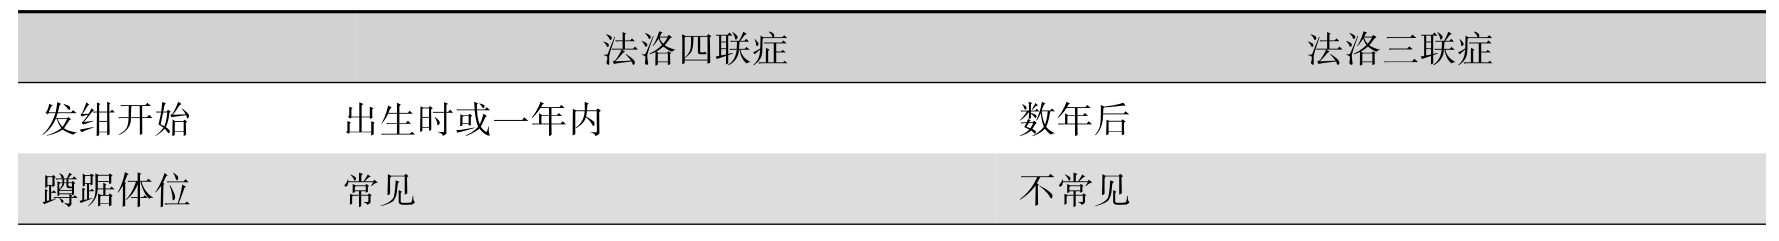
\includegraphics[width=\textwidth,height=\textheight,keepaspectratio]{./images/Image00093.jpg}\\
 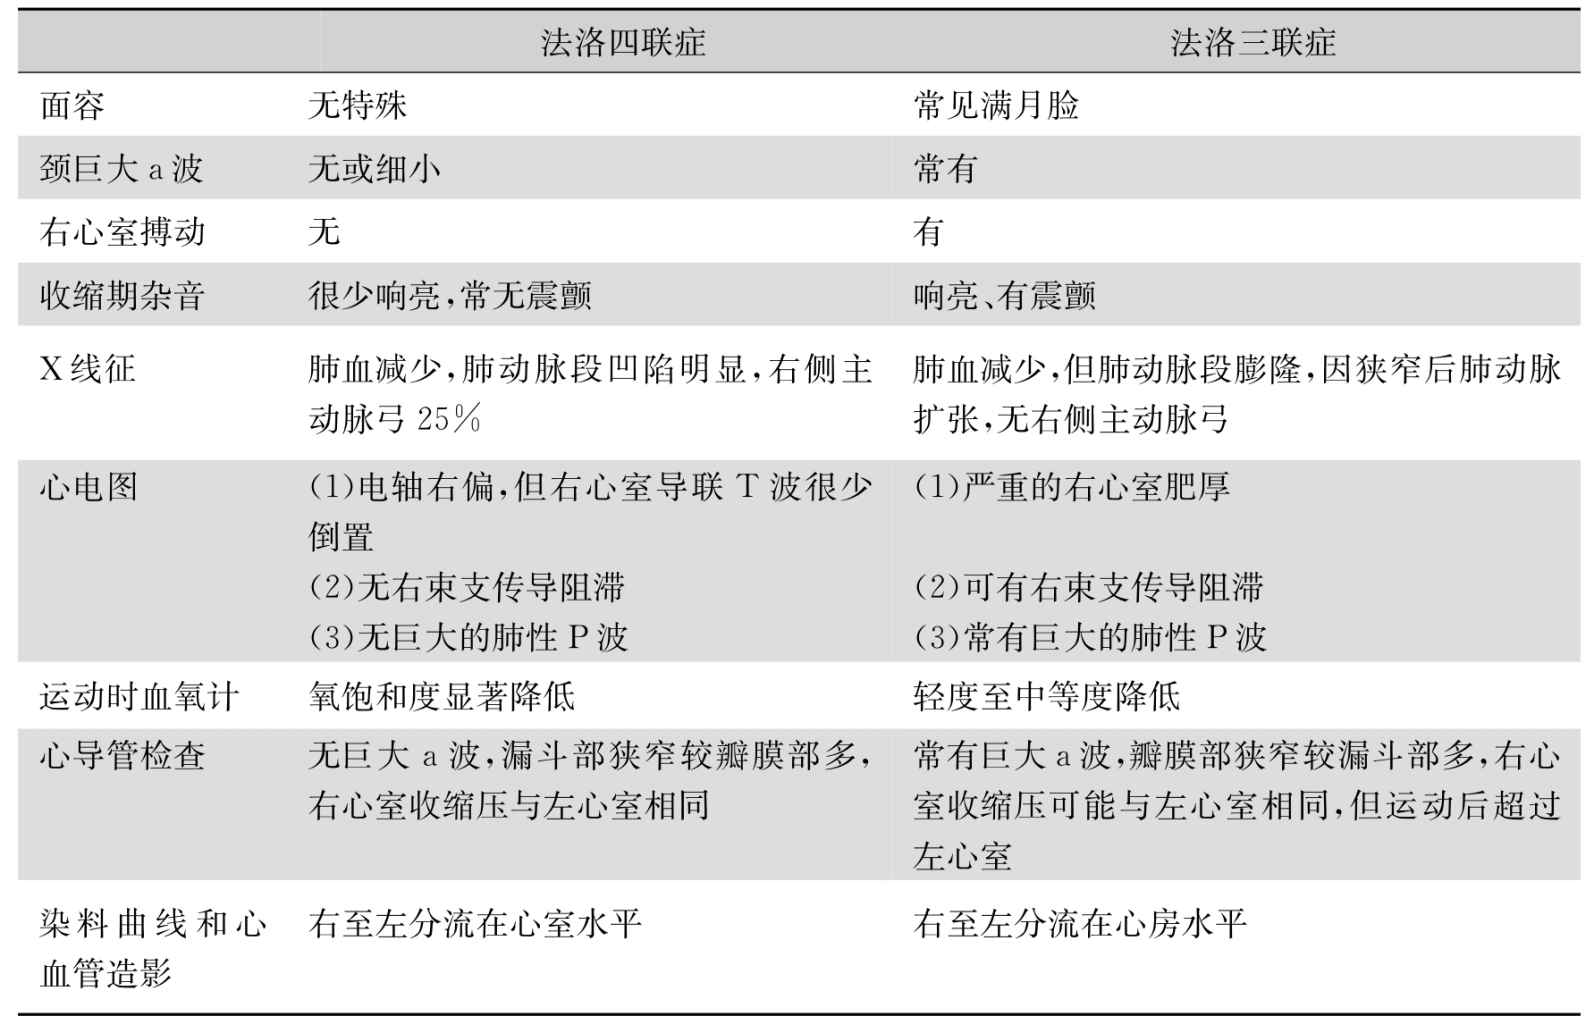
\includegraphics[width=\textwidth,height=\textheight,keepaspectratio]{./images/Image00094.jpg}
 \end{longtable}

\hypertarget{text00120.htmlux5cux23CHP14-5-1-5-1-1-2}{}
2.肺动脉瓣闭锁

本病通常合并室间隔缺损。如合并室间隔缺损,则与法洛四联症很相似。区别在于本病是没有不发绀的,且发绀常显著。另一区别点是本病无肺动脉瓣区喷射型收缩期杂音;如病儿有重度发绀而无此杂音,提示本病的诊断。常有柔和的连续性杂音存在,乃由于动脉导管未闭或支气管动脉、肺动脉交通支所致;如连续性杂音位于右侧,则提示后者。X线检查显示升主动脉凸出,提示本病的诊断;除有支气管动脉扩张所致的斑点状肺门阴影之外,其表现与法洛四联症很相似。心血管造影可显示明显的支气管动脉-肺动脉交通支,而无主肺动脉的影像;注入造影剂于右心室中,造影剂通过室间隔缺损而使主动脉显影。心导管检查发现导管行径不能从右心室进入肺动脉。如有室间隔缺损存在,左、右心室与主动脉的收缩压均相同。病儿大都死亡于婴幼期。

\hypertarget{text00120.htmlux5cux23CHP14-5-1-5-1-1-3}{}
3.艾森曼格综合征

伴有分流在心室水平的本综合征与法洛四联症的鉴别要点是:①前者肺动脉近侧分支显著扩张,而后者肺野异常清朗,肺纹理稀少;②前者肺动脉段膨隆,而后者多凹陷,仅少数呈肺动脉瓣狭窄后膨隆;③前者肺动脉瓣第二音亢进,而后者常减弱;④前者的发绀出现较晚和较轻,而后者的发绀出现甚早且较重;⑤右心导管检查前者有肺动脉高压,而后者肺动脉压力降低。

\hypertarget{text00120.htmlux5cux23CHP14-5-1-5-1-1-4}{}
4.永存动脉干合并肺动脉高压

参考本节下文。

\hypertarget{text00120.htmlux5cux23CHP14-5-1-5-1-1-5}{}
5.大血管错位合并肺动脉瓣狭窄

参考本节下文。

\hypertarget{text00120.htmlux5cux23CHP14-5-1-5-1-1-6}{}
6.单心室

参考本节下文。

\subparagraph{(二)大血管错位}

\hypertarget{text00120.htmlux5cux23CHP14-5-1-5-1-2-1}{}
1.完全性大血管错位

本病时主动脉在前出自右心室,肺动脉在后出自左心室,其成因乃由于心球在发育时未作正常的旋转所致。病婴只有在体循环与肺循环之间有分流存在时才能存活。病婴出生时即有重度发绀。发绀、心脏增大与心力衰竭,是大血管错位最常见的表现。但有些病婴可仅有轻度发绀。约1/4病例可以无心杂音。典型的Roger杂音(胸骨左缘第三、四肋间粗糙的收缩全期杂音)伴有震颤,起因于室间隔缺损。如合并动脉导管未闭,连续性杂音也很难听到。肺动脉瓣区第二音响亮,此增强的第二心音起源于主动脉瓣,但由于大血管错位而在胸骨左缘听到。心电图常显示高度右心室肥厚,但有时显示双侧心室肥厚。后前位X线检查显示大血管根部特别狭窄,双侧心室增大,主要是右心室增大,心影呈“横置的蛋形”。左前斜位显示大血管根部宽阔(因主动脉错位在前,肺动脉错位在后)。如无脉动脉瓣狭窄或三尖瓣闭锁存在,而有恒定的肺充血与肺动脉弓缺如,高度提示本病。选择性心血管造影可显示主动脉瓣的位置异常高,与肺动脉瓣同一水平,造影剂从右心室进入主动脉,主动脉在前。右心导管检查导管行径从右心房至右心室,随即进入主动脉。

\hypertarget{text00120.htmlux5cux23CHP14-5-1-5-1-2-2}{}
2.部分大血管错位

部分大血管错位有两种类型:

\hypertarget{text00120.htmlux5cux23CHP14-5-1-5-1-2-2-1}{}
(1)主动脉错位合并肺动脉骑跨:

大血管可呈90°或180°逆时针转位。最常见的类型是Beuren型,这时主动脉在肺动脉之前从右心室分出,肺动脉骑跨于左右两心室之上。较少见的类型是Taussig-Bing综合征,主动脉从右心室分出,稍后于肺动脉,肺动脉仍骑跨于两侧心室之上。此两种畸形均合并室间隔缺损,临床病象与全部大血管错位相似,表现为室间隔缺损合并肺动脉高压与发绀、收缩全期杂音、肺动脉瓣区第二音响亮与肺充血。心血管造影有助于鉴别肺动脉起始于两侧心室。

\hypertarget{text00120.htmlux5cux23CHP14-5-1-5-1-2-2-2}{}
(2)右心室双重出口:

本畸形时主动脉与肺动脉均从右心室分出。主动脉的位置常稍后,经由室间隔缺损接受左心室的血液。临床表现类似伴有发绀的室间隔缺损;又如伴有肺动脉瓣狭窄,则可类似法洛四联症。心电图表现与心内膜垫缺损过渡型相同(参见第47节),是提示诊断的重要临床线索。选择性左心室血管造影显示室间隔缺损是唯一的左心室出口;右心室血管造影在侧位片上显示主动脉与肺动脉在同一平面,主动脉瓣的位置高于正常的位置。

\subparagraph{(三)完全性肺静脉畸形引流}

引流入右心房时,须有房间隔缺损或未闭的卵圆孔与左心房沟通,以供应体循环的氧合血。大多数患者死于幼年,有些可存活至成年。心脏病征通常与房间隔缺损相同:右心室抬举性搏动、肺动脉搏动、肺动脉瓣区喷射型收缩期杂音与第二心音分裂宽。功能性舒张中期杂音也常听到。但与单纯的房间隔缺损也有所不同;①可有轻度发绀;②1/4病例在主动脉瓣区可听到连续性杂音,吸气时增强,由于其下有大的异常静脉通路之故。周围动脉搏动减弱。心电图表现与房间隔缺损相同。如伴有左侧上腔静脉,合并左侧无名静脉与右侧上腔静脉,X线检查心影呈“8”字形或“大小两块合拢的面包形”。右心房、右心室与肺动脉均扩大,肺充血。选择性心血管造影可显示异常肺静脉的解剖学位置。右心导管检查发现主动脉、肺动脉和四个心腔的血氧含量均相同。

\subparagraph{(四)三尖瓣闭锁}

患本病的病婴通常死亡于婴幼期,但有些患者可存活至20岁,特别是合并大血管错位时。国内有少数病例报告。本病可区分为两种类型:

Ⅰ型:三尖瓣缺如,右心房扩大,须有房间隔缺损才能生存。常合并肺动脉瓣膜部或漏斗部狭窄伴有肺动脉发育不良。肺缺血。

Ⅱ型:伴有大血管错位(约占1/4病例)。右心室的心腔必然存在,因室间隔缺损是维持生存所必需的。静脉血从右心房经由房间隔缺损进入左心房。左心房血液进入左心室后,一部分经由肺动脉进入肺内,一部分通过室间隔缺损进入右心室。右心室血液进入主动脉。肺充血。

Ⅰ型有重度发绀、杵状指(趾)与蹲踞体位。缺氧性发作常见。如合并大血管错位,发绀常轻微。如有室间隔缺损,常出现收缩全期杂音与震颤。有时也可出现连续性杂音,较常由于动脉导管未闭引起,少数由于支气管动脉-肺动脉交通支引起。如发绀患者伴有左心室肥厚的心电图,对本病有确实的诊断意义。常有明显的肺性P波。这种情况不常见于其他原因的左心室肥厚。

X线检查在Ⅰ型有左心室增大,合并右心房增大、肺动脉发育不良与肺缺血。心血管造影显示造影剂从右心房→左心房→左心室。左心室显影常早于右心室,右心室常不显影。

发绀合并左心室增大不仅见于三尖瓣闭锁,还可见于永存动脉干,但这时发绀常不严重。永存动脉干与三尖瓣闭锁不同,可有不完全性右束支传导阻滞。右心导管检查在三尖瓣闭锁的诊断上甚少需要。导管的尖端在扩大的右心房内不能进入右心室,但常容易经由房间隔缺损进入左心房,左心房血氧含量低,如同右心房。

\subparagraph{(五)永存动脉干}

如胚胎期心球隔不发育,则形成永存动脉干。由于心球隔参与室间隔的发育,故本病有不同程度的室间隔缺损。肺动脉以单支的形式从动脉干的后壁分出,或从动脉干任何一侧独自分出。临床表现主要是有大的左至右分流合并轻度发绀。出生后数月即有发育不良与充血性心力衰竭。常见有心前胸壁隆起与进行性心脏增大。在出生一个月之后,70\%病例在胸骨左缘第三、四肋间出现收缩期杂音,偶伴震颤,与大的室间隔缺损相同。第二心音是单一的,且亢进。大多数病婴生存不超过6个月。如发育不良的肺动脉从动脉干分出,又或发生肺动脉高压症,则寿命较长。偶尔活至中年。如发生肺动脉高压症,表现为艾森曼格综合征的病象,或类似法洛四联症。心电图无特别,胸导联显示双侧心室肥厚可能是最常见的表现。X线检查显示中等度至高度心脏增大,心影无特别。胸透时可见肺动脉分支充血与有力的搏动。如左肺动脉的高度接近主动脉弓的水平,应考虑永存动脉干。心导管检查时导管行径可经由动脉干进入一支肺动脉。所有病例均有动脉血氧饱和不足,而当肺动脉高压时可更严重。从动脉干的近心端注入造影剂,可显示动脉干和肺动脉的起点。

\subparagraph{(六)单心室单心室(二房三腔心)}

本病时室间隔完全缺如,而房间隔发育正常。如兼有房间隔缺损,则称为二腔心。二尖瓣与三尖瓣正常地开口于共同的单心室,但也可伴有二尖瓣畸形。约3/4病例有呼吸困难。幼年时期充血性心力衰竭也常见。发绀常存在,但可轻微。如合并肺动脉瓣狭窄则有重度发绀。X线检查心脏仅轻度或中等度增大,心影无特别。如无大血管错位,心影与大的室间隔缺损相似。如合并肺动脉瓣狭窄,则类似法洛四联症。心电图有几种类型高度提示本病的诊断:①右胸导联可呈QR型,并有右心室肥厚的征象,左胸导联s波深而常无Q波;②无合并大血管错位的单心室,其所有的胸导联上s波深、T波直立,虽然电压可有些改变,但波形改变甚少;③胸导联上如有等相综合波(equiphasic
complexes),也提示本病的诊断。心血管造影可显示大血管错位与主动脉瓣位置升高。造影剂充盈一个巨大的单心室,主动脉与肺动脉同时显影。肺动脉瓣狭窄也可显示出来。只靠右心导管检查不能区别单心室与很大的室间隔缺损。

据近年国内一组单心室73例报道,单心室易并存多种心内畸形及心脏异位。因而,术前应综合心电图、超声心动图、心血管造影等作出判断。手术所见则为更确实的诊断。

\paragraph{二、迟显性发绀}

如发绀不在出生时出现,而在出生以后逐渐出现,称为迟显性发绀。如发绀类先天性心脏病患者已除外周围性发绀及血液在肺内氧合不足等所致的发绀,则高度可能有右至左的分流存在。

有些早显性发绀的先天性心脏病,其发绀也可为迟显性;反之亦然。

\subparagraph{(一)艾森曼格病与艾森曼格综合征}

艾森曼格(Eisenmenger)病是指大的高位室间隔缺损伴主动脉右位而无肺动脉瓣狭窄,有肺动脉高压,肺血管阻力处于或高出体循环水平,血流因而经由右心室至左心室,或主要地经由右心室至左心室,分流方向相反。艾森曼格综合征是指任何先天性心血管畸形所致的左右两侧心相沟通,引起与艾森曼格病相同的血流动力学改变,相反方向的分流常经由房间隔缺损、室间隔缺损或未闭的动脉导管,较少见的情况下由于主-肺动脉隔缺损、永存动脉干、大血管错位等。呼吸困难推测主要是由于未饱和的氧合血作用于外周化学感受器所致。心输出量减少引起心绞痛与劳动后晕厥。通常因有肺梗塞而致咯血;咯血可严重,甚或引起死亡。

体征:不论分流在什么部位,通常有下列的体征:

1.桶形胸首先由于肺血流量增加,以后由于肺血管阻力增高所引起。

2.中心性发绀除房间隔缺损之外,常在幼年时期出现。

3.由于右心室肥厚与主肺动脉扩张,可触及搏动。

4.常有肺动脉瓣区柔和的喷射型收缩期杂音,且常继以响亮的喷射附加音。

5.肺动脉瓣区第二音是单一的,或有互相接近的心音分裂、肺动脉瓣组成部分响亮且可触及。

6.右心房扩大,可伴有右心房第四心音。

7.由于相对性肺动脉瓣关闭不全,可出现史氏杂音。

8.如发生右心室衰竭,三尖瓣环扩大,可引起相对性三尖瓣关闭不全,常在三尖瓣区出现收缩全期杂音。

9.颈静脉压升高,a波明显。

10.心输出量低(由于肺血流梗阻)导致周围动脉搏动减弱。

X线检查:显示由于肺动脉高压导致主肺动脉及其近侧分支的显著扩张,但两肺外周纹理稀少,肺野异常清朗。选择性心血管造影可显示缺损的部位,但在艾森曼格综合征时有很大的危险性。

心电图检查:由于有心房肥大而出现肺性P波,心室综合波显示右心室肥厚。

右心导管检查:肺动脉血压与体循环动脉血压相等。除可证明右至左分流之外,还常可发现小量的左至右分流。

引起艾森曼格综合征的三种先天性心脏病的互相鉴别见表\ref{tab14-3}。第二心音的听诊有助于缺损部位的初步鉴别:动脉导管未闭时第二心音分裂互相接近,随呼吸运动而正常地变动(即深吸气末期心音分裂较宽);室间隔缺损时第二心音是单一的;房间隔缺损时第二心音分裂宽,吸气时固定不变。

\begin{table}[htbp]
\centering
\caption{通常引起艾森曼格综合征的三种缺损的鉴别}
\label{tab14-3}
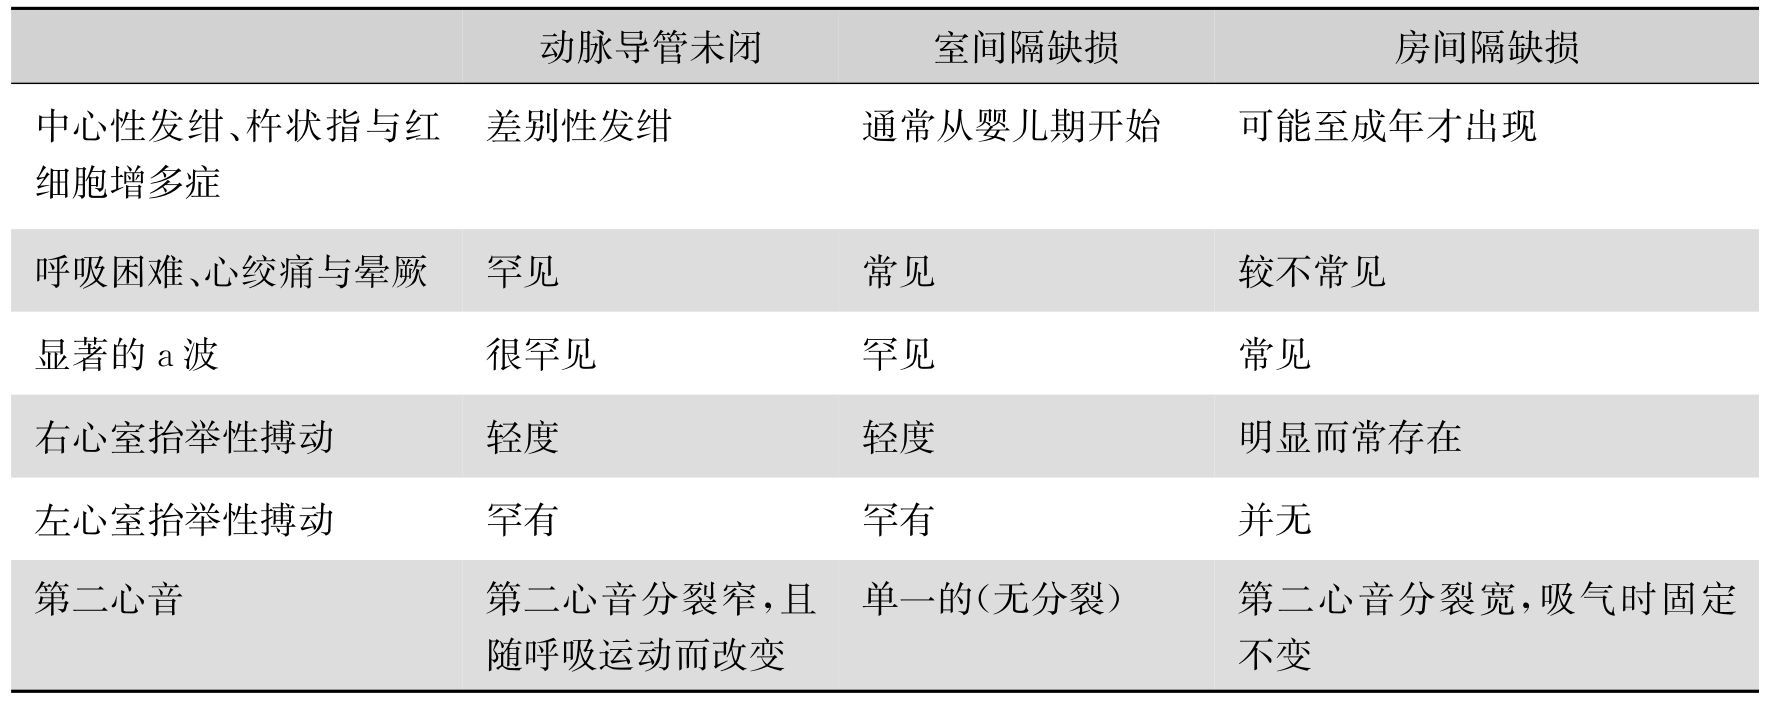
\includegraphics[width=5.89583in,height=2.33333in]{./images/Image00095.jpg}
\end{table}

\subparagraph{(二)法洛(Fallot)三联症}

肺动脉瓣狭窄合并房间隔缺损与分流方向相反,称为法洛三联症。分流常经由扩大的卵圆孔,真正的房间隔缺损罕见。出生后可能即出现持续性发绀,但发绀常较迟出现,偶尔在青春期后或成年才出现。国内报告法洛三联症一组10例中,8例有发绀。杵状指(趾)和红细胞增多症可伴随发绀而出现。发绀患者可出现蹲踞体位,但不如法洛四联症的常见。X线表现心脏增大显著,主肺动脉明显凸出,肺野清晰,无右侧主动脉弓。本症与法洛四联症的鉴别可有困难,除非导管尖端能通过缺损口。表\ref{tab14-2}可供二者鉴别的参考。

\subparagraph{(三)爱泼斯坦畸形合并卵圆孔未闭或房间隔缺损}

在爱泼斯坦畸形时,三尖瓣瓣叶变形和向下移进右心室;在瓣膜游离缘的近端,心室的心房化部分异常菲薄,而远端的右心室壁的厚度则正常。心脏的大小和形状,与三尖瓣向下移位的程度以及有作用的右心室和心房化部分的比例有关。肺血流量减少提示肺动脉瓣狭窄。发绀是由于血液通过未闭合的卵圆孔或房间隔缺损,从右至左分流。本病国内有少数病例报告。

常见的症状是呼吸困难,但患者可以多年无症状。常有显著的发绀和轻度杵状指。发绀常迟显,但可于出生时出现。常有乏力,但蹲踞体位不常见。较常有阵发性心律失常和猝死。偶尔无明显的循环障碍,无发绀和无症状。

体格检查发现显著的心脏增大,但心脏搏动减弱。听诊特征是三音心律或四音心律,第一心音迟延,第二心音分裂宽,肺动脉瓣关闭音减弱,第四心音明显。可能给人以奔马律的印象,但心率不快。沿胸骨左缘,在心尖区或偶尔弥漫地在心前区有收缩全期杂音,可能由于三尖瓣关闭不全或经室间隔缺损的从左至右分流。收缩期杂音也可能由于肺动脉瓣狭窄或动脉导管未闭所致。很多病例有心尖区低调舒张期杂音,可能由于通过二尖瓣的血流增加。

X线检查发现心脏增大,特别是右侧(巨大的右心房)。如右至左分流量大,则主肺动脉段凹陷,肺动脉纹理减少。X线透视对诊断甚有帮助。在后前位可见有心房搏动。于左前斜位在上方仍见右心房搏动;但心房化的右心室边缘的搏动却显著减弱乃至消失。在右前斜位可见到搏动减弱和右心室流出道搏动较正常的分界点。

心电图常显示右束支传导阻滞和右心室导联的QRS综合波低电压。P波高而尖。P-R间期延长。有些患者有预激综合征,或出现室上性和室性心律失常。

这些患者在进行心导管检查和心血管造影时可发生严重的心律失常,必须充分估计其危险性。肺动脉和右心室收缩压低,心输出量可能减少。在压力曲线显示右心房压力波形的导管位置,心内心电图显示右心室综合波,有重要的诊断意义。

心血管造影可能辨别心房化的变薄的右心室壁和三尖瓣的瓣叶游离缘所在的不规则区。不可错误地认为三尖瓣位于房室沟。在心房的水平有右至左的分流。爱泼斯坦畸形在X线检查时,由于心底部狭窄、心影呈球形、肺野清朗,可被误诊为心包积液;此外,尚须与慢性右心衰竭、三尖瓣闭锁、重度肺动脉瓣狭窄合并房间隔缺损与右至左分流等相鉴别,主要根据上述检查。超声心动图为最有意义的诊断工具。

\subparagraph{(四)先天性肺动脉瓣狭窄}

有四种临床类型:①轻度;②中等度;③重度;④肺动脉瓣狭窄兼有分流。

轻度与中等度肺动脉瓣狭窄无发绀。重度肺动脉瓣狭窄可有发绀,发绀为周围性。

肺动脉瓣狭窄合并右至左分流可出现发绀。发绀为迟显性,通常出现于青年时期。发绀初时可仅在劳动后出现。如右至左分流经由室间隔缺损,血流动力学改变类似法洛四联症,但并无主动脉骑跨。如肺动脉瓣狭窄严重,右心房压力高于左心房,则阻碍卵圆孔的闭合。患者出生时即有发绀(法洛三联症)。肺动脉瓣狭窄的诊断参见第47节。

\protect\hypertarget{text00121.html}{}{}

\subsection{44.2 周围性发绀}

周围性发绀是由于血液通过周围循环毛细血管时,因血流速度缓慢、淤滞、组织耗氧率增加,致血氧未饱和度增加(达到或超过6.5容积\%),因而产生发绀。这种情况可见于全身性或局限性病变。

周围性发绀应与中心性发绀相鉴别。周围性发绀通常由于血液淤滞,因此常出现于肢体的下垂部分及周围部位,例如肢端与颜面;这些部位是冰冷的。反之,中心性发绀为全身性,除四肢及颜面之外,也累及黏膜(包括口腔黏膜)及躯干的皮肤,皮肤是温暖的。若难以鉴别,可按摩和加温发绀的耳垂或肢端,使之温暖。如为周围性发绀,则皮肤温暖后,发绀即消失;如发绀不消失,则为中心性发绀。

\subsubsection{44.2.1 全身性疾病}

\paragraph{一、淤血性周围性发绀}

充血性心力衰竭、慢性缩窄性心包炎、三尖瓣膜病等,均可导致体循环血液淤滞、血流速度减慢,从而引起发绀。

\paragraph{二、缺血性周围性发绀}

休克时心输出量减低,周围循环供血减少,毛细血管内血液淤滞,可以出现发绀。

\paragraph{三、其他疾病的周围性发绀}

\subparagraph{(一)冷凝集现象伴有手足发绀症}

冷凝集现象伴有手足发绀症冷凝集现象的产生,乃由于患者血清中含有大量的冷凝集素。这种情况可见于肺炎支原体肺炎的患者,遇天气寒冷时,可使自身红细胞在肢端毛细血管内凝集,致引起局部血液循环障碍与发绀。诊断可根据患者血清内的高度冷凝集素效价。国内文献报告,在一些无肺炎支原体肺炎的人(绝大多数为农业劳动者)、冷反应自身免疫溶血性贫血患者也可出现此种现象。

先天性梅毒引起的雷诺现象,与溶血素有关(参见第113.2.1节)。

\subparagraph{(二)冷球蛋白血症}

冷球蛋白(cryoglobulin)在低温时可自行凝固。但大量的冷球蛋白血症几乎只见于多发性骨髓瘤,文献报告有因此而引起广泛性紫癜、雷诺现象及视网膜静脉血栓形成者。如做血细胞容积测定,可见红细胞层之上有灰黄色胶样物质层,高达10mm,此即冷球蛋白。本病属单克隆免疫球蛋白病范畴。

\subparagraph{(三)真性红细胞增多症}

本病的三大特征是:红细胞增多、皮肤色紫红与肝脾大。患者口唇与肢端可出现发绀,多由于血液黏稠度过高,血流缓慢,在周围组织耗氧过多,以及血红蛋白本身的改变,致血红蛋白与氧结合的能力降低引起。

\subsubsection{44.2.2 局部血流障碍性疾病}

周围局部组织中由于动脉供血不足、静脉回流受阻或自主神经功能紊乱等所引起的局限性发绀,成为内科疾病鉴别诊断上一项较常见的课题,下文将分别讨论之。

\paragraph{一、血栓闭塞性脉管炎}

本病的主要表现为持续性或阵发性肢端疼痛,也可引起间歇性跛行、肢端发绀等。

\paragraph{二、雷诺病}

雷诺(Raynaud)病是一种功能性疾病,病因未明,症状主要由于周围小血管(小动脉、小静脉)痉挛所引起。国内病例报道不多。发病年龄多在20~30岁之间,女性与男性发病比率约为10∶1。

本病的特征是阵发性、双侧对称性肢端发白、麻木与发绀。发病部位主要限于手指与足趾,常因情绪激动或寒冷刺激而诱发。严重者可引起肢端坏疽。发作经过可分为三个阶段:局部缺血期、局部窒息期与缓解期。如作冷水试验,将罹患肢端浸于4℃(或温度稍高)的冷水中1分钟,可诱发典型的雷诺现象发作:苍白→发绀→变红,每期持续4~10分钟不等。两手握拳1.5分钟后,在弯曲状态下放开,也可出现相同的现象(握拳试验)。作皮肤紫外线照射试验时,皮肤对紫外线照射红斑反应减弱,且两侧肢端的反应不同,提示周围血管舒缩障碍。患肢的动脉搏动并无减弱或消失,病变主要累及肢端,双侧同时发病,故与血栓闭塞性脉管炎有所不同。

本病的诊断根据是:①患者有上述的临床表现;②除外各种原因所致的雷诺现象,特别是结缔组织疾病所致的雷诺现象。

\paragraph{三、肢端发绀症}

肢端发绀症(acrocyanosis)以年轻女性多见,是一种自主神经症,患者常有皮肤划痕症、手心多汗等自主神经功能紊乱现象。肢端常有冷感与发绀,寒冷可使症状加重,病变也常累及双手,且多见于年轻女性,须与雷诺病相区别。在肢端发绀症时,不能见到典型的雷诺现象(苍白→发绀→变红),也无皮肤苍白的现象。在雷诺病时,发绀往往限于指、趾等狭小的范围。而在肢端发绀症时,持续的、均匀的发绀可出现于整个手部与腕部,甚少出现于足部;暴露于冷空气中虽可使症状加剧,但在温暖环境中常不能使之减轻或消失。且从未见有溃疡形成或坏疽。

\paragraph{四、肢体动脉硬化所致的雷诺现象}

动脉粥样硬化是四肢动脉疾病常见原因之一。在55岁以前少见,而糖尿病性动脉硬化则发病较早。病变常侵及下肢的胫后动脉与足背动脉的终末分支,如引起供血不足,则患者常觉有足趾麻木、刺痛与烧灼感,足部较正常时为凉,足趾发白。胫后动脉与足背动脉搏动微弱或未能触知,是诊断上有意义的病征。患者在动脉完全阻塞之前可出现间歇性跛行。动脉造影可发现动脉狭窄的征象。

\paragraph{五、结缔组织病所致的雷诺现象}

硬皮病与系统性红斑狼疮可发生雷诺现象,有些病例且为早期主要症状,出现于典型病象显露之前,可引起鉴别诊断上的困难。系统性硬皮病具有皮下组织钙质沉着、雷诺现象、指硬皮和毛细血管扩张者,称为CRST综合征。

雷诺现象对结缔组织病的诊断意义在于其常见且早发,有早期诊断意义。国内报告一组混合性结缔组织病,主要症状依次为雷诺现象83.3\%,关节痛(炎)80\%,面部及手指肿胀各60\%,手指硬化50\%,肌炎46.7\%。

\paragraph{六、心房黏液瘤}

雷诺现象作为心房黏液瘤的主要症状罕见。国内仅有一例报告左心房黏液瘤以晕厥和雷诺现象为早期症状。其原因可能由于瘤体脱落的碎片或瘤体表面血栓脱落所发生的小栓塞,以及瘤体阻塞血流使周围组织缺氧而致肢端小动脉痉挛所引起。摘除瘤体后雷诺现象亦消除。

\paragraph{七、振动病}

本病也称职业性雷诺现象。使用振动工具(特别是链锯)和转动工具(如砂轮),可引起本病。寒冷常为促发或加重症状的因素。

\paragraph{八、胸廓出口综合征}

此综合征多发生于30~50岁之间,女性发病率较高。如臂丛神经受压,则引起肩胛部疼痛及手臂内侧放射痛。锁骨下动脉受压时,手部皮肤可出现厥冷、苍白与发绀现象(参见第149节)。

\paragraph{九、网状紫斑}

网状紫斑国内有少数病例报告。患者多为女性,其特点是皮肤呈网状或斑状青紫现象。病变多发生于下肢,但也可累及上肢、躯干和颜面等部位。患肢常有发冷、麻木与感觉异常,有时或酸痛。温度与位置对紫斑有一定的影响。暴露于寒冷环境中或取下垂位置时,斑纹即明显;加温及(或)将患肢抬高后,斑纹常可逐渐减轻或甚至消失。严重病例可发生脚趾溃疡或坏疽。

本病临床上可分为三型:

1.大理石样皮斑
是较轻的一种,患者以女性较多。受凉后皮肤出现紫红色网纹,纹理较细,温暖后即渐消失。

2.特发性网状紫斑
紫红色斑纹较为明显,且范围较广,虽在温暖环境中也不完全消失。

3.症状性网状紫斑
常与结核病、慢性肝炎、结节性多动脉炎、结节性红斑、梅毒等并存。有时斑纹可高出皮面呈索条状,在这些索条中还可触到一些小结节。

\hypertarget{text00121.htmlux5cux23CHP14-5-2-2-10}{}
十、局部静脉病变

因下肢静脉曲张、血栓性静脉炎等所致的患肢局部血液循环障碍,均可引起轻度的局限性发绀。上腔静脉阻塞也能引起颜面及上肢发绀和水肿。

\protect\hypertarget{text00122.html}{}{}

\section{参考文献}

1.于秀章.原发性肺动脉高压症------附6例报告.中华内科杂志,1963,11:43

2.王瑞康,等.原发性肺动脉高压症(附8例病例报告).天津医药,1981,9:14

3.赵小平.原发性肺动脉高压症诊断的探讨.中华内科杂志,1986,25:84

4.丁嘉安.肺动静脉瘘.中华外科杂志,1980,18:33

5.李国业,等.完全性肺静脉畸形引流2例报告.新医学,1980,11(11):583

6.郑道声.三尖瓣闭锁二例报告.中华内科杂志,1963,11:491

7.朱瑞珍.法鲁氏三联症-附10例临床分析.中华内科杂志,1963,11:517

8.郑道声.法乐氏五联症39例临床分析.中华心血管病杂志,1985,13:40

9.郑更生.埃勃斯坦氏畸形四例报告.中华内科杂志,1963,11:587

10.胡旭东,等.Ebstein畸形.中华心血管病杂志,1980,8(4):273

11.梅先受.原发性非典型肺炎并发手足发绀症一例报告.中华内科杂志,1957,4:584

12.曾庆余.冷凝蛋白血症的神经系统表现.中华内科杂志,1984,23:746

13.叶仲等.可逆性低温血凝症具有周围循环症状------附10例报告.中华内科杂志,1963,11:589

14.俞国瑞.雷诺氏病二例.中华内科杂志,1958,6:386

15.湖南医学院第一附属医院内科.全身性红斑狼疮100例临床分析.中华内科杂志,1978,17(5):365

16.欧阳钦.临床诊断学.人民卫生出版社,2005,33-35

17.杜立中.新生儿常见疾病的鉴别诊断:新生儿青紫的鉴别诊断学.中国实用儿科杂志,2001,16(3):129-1311

18.王吉耀.内科学.第2版.人民卫生出版社,2010,370-385

19.黄冰生,等.紫绀的病因与鉴别诊断.新医学,2005,36:4

20.王忻,等.新生儿紫绀型先天性心脏病26例早期诊断分析.中国实用儿科杂志,2009(5):393-394

21.徐仲英,等.成人先天性心脏病临床对策.中国实用内科杂志,2013(4):272-276

22.姚青,等.先天性心脏病相关性肺动脉高压的临床诊断与评估.心血管病学进展,2013,34(5):599-603

23.韩智群,等.误服亚硝酸盐中毒急诊诊治体会.临床急诊杂志,2012,13(6):444-445

24.逯军.关注新生儿心血管疾病诊疗.中国新生儿科杂志,2011,16(3):150-153

25.李寒,等.上腔静脉-右肺动脉分流术治疗三尖瓣闭锁.中国胸心血管外科临床杂志,2010,17(1):73-74

26.邹捍东,等.丙泊酚、咪达唑仑对小儿紫绀型先天性心脏病体外循环心内直视术的心肌保护作用.中华医学杂志,2007,87(33):2309-2312

27.齐运平.隔夜菜汁致高铁血红蛋白血症13例分析.中国新生儿科杂志,2007,22(5):308

\protect\hypertarget{text00123.html}{}{}

